\documentclass[solution, letterpaper]{cs121}

\usepackage{tikz-qtree}
\usepackage{graphicx}
\usepackage{color}
\usepackage{amsfonts}
\usepackage{amsmath}
\usepackage[english]{babel}
\usepackage[utf8]{inputenc}
\usepackage{ae,aecompl}

% allow metapost figures to be included inline
% note: you must invoke latex using:
%
%     pdflatex -shell-escape <inputfile>
%
% to allow it to invoke external commands. See the very end of the
% document as well.
\usepackage{emp,ifpdf}
\usepackage{graphicx}

% convert metapost figures to .eps or .pdf automatically when
% including them
\ifpdf\DeclareGraphicsRule{*}{mps}{*}{}\fi

% include the metapost macros
\empprelude{input boxes; input theory}

%% Please fill in your name and collaboration statement here.
%\newcommand{\studentName}{Renzo Lucioni and Daniel Broudy}
%\newcommand{\collaborationStatement}{I collaborated with...}
\newcommand{\solncolor}{red}
\begin{document}

% create a metapost file for figures to be dumped to.  It's easiest
% to use a single file for all the figures in the document
\begin{empfile}

\header{4}{April 12, 2013, at 12:00 PM}{}{}

%%%%%%%%%%%%%%%%%%%%%%%%%%%%%%%%%%%%%%%%%%%%%%%%%%%%
\problem{14} %1

\subproblem %a
The diagram below illustrates the directed graph structure of the network.

\begin{center}
\begin{emp}(0,0)
  % it's good practice to pick a basic size unit and make all your
  % distances relative to that unit
  u := 2cm;
  ubernodes;
  % create a node, and position its center at the origin
  node.q1(btex $MAI$ etex); q1.c = origin;

  % position the other nodes relative to it
  node.q2(btex $NAI$ etex); q2.c = q1.c + (1.5u,0);
  node.q3(btex $RD$ etex); q3.c = q1.c + (3u,0);
  node.q4(btex $VRAS$ etex); q4.c = q1.c + (0.75u,-1.5u);
  node.q5(btex $SMOS$ etex); q5.c = q1.c + (2.25u,-1.5u);
  node.q6(btex $VP$ etex); q6.c = q1.c + (1.5u,-3u);

  % mark q1 as a start node
  %makestart(q1);

  % mark q4 as an accept node
  %makefinal(q1);

  % draw the nodes
  drawboxed(q1,q2,q3,q4,q5,q6);

  edge(q1,q4,right,btex etex);
  edge(q2,q4,right,btex etex);
  edge(q3,q5,right,btex etex);
  edge(q4,q6,right,btex etex);
  edge(q5,q6,right,btex etex);

\end{emp}
\end{center}

The following describes a parameterization of the noise in the causal effects of the above dependencies. WE NEED TO PROVIDE PRIOR PROBABILITY TABLES AS PART OF THE PARAMETRIZATION
\begin{equation*}
\resizebox{1\hsize}{!}{$P(RD,SMOS,VRAS,MAI,NAI,VP) = P(MAI)P(NAI)P(RD)P(VRAS | MAI, NAI)P(SMOS | RD)P(VP | VRAS, SMOS)$}
\end{equation*}

The nodes $MAI$, $NAI$, and $RD$ are binary attributes which are not conditional on any other attributes. They are each associated with a probability vector.
\begin{center}
\begin{tabular}{ l |c r }
   $MAI = 0$ & $MAI = 1$ \\
   \hline
  .6 & .4 \\
\end{tabular}
\end{center}

\begin{center}
\begin{tabular}{ l |c r }
   $NAI = 0$ & $NAI = 1$ \\
   \hline
  .3 & .7 \\
\end{tabular}
\end{center}

\begin{center}
\begin{tabular}{ l |c r }
   $RD = 0$ & $RD = 1$ \\
   \hline
  .2 & .8 \\
\end{tabular}
\end{center}

$VRAS$ is conditional on $MAI$ and $NAI$ and is associated with the following conditional probability tables.
\begin{center}
\begin{tabular}{ l |c r }
   $VRAS = 0$ & $NAI = 0$ & $NAI = 1$ \\
   \hline
  $MAI = 0$ & .5 & .2 \\
  $MAI = 1$ & .2 & .1 \\
\end{tabular}
\end{center}

\begin{center}
\begin{tabular}{ l |c r }
   $VRAS = 1$ & $NAI = 0$ & $NAI = 1$ \\
   \hline
  $MAI = 0$ & .1 & .2 \\
  $MAI = 1$ & .2 & .5 \\
\end{tabular}
\end{center}

$SMOS$ is conditional on $RD$ and is associated with the following conditional probability table.
\begin{center}
\begin{tabular}{ l |c r }
   & $RD = 0$ & $RD = 1$ \\
   \hline
  $SMOS = 0$ & .8 & .2 \\
  $SMOS = 1$ & .1 & .9 \\
\end{tabular}
\end{center}

$VP$ is conditional on $VRAS$ and $SMOS$ and is associated with the following conditional probability tables.
\begin{center}
\begin{tabular}{ l |c r }
   $VP = 0$ & $SMOS = 0$ & $SMOS = 1$ \\
   \hline
  $VRAS = 0$ & .7 & .1 \\
  $VRAS = 1$ & .1 & .1 \\
\end{tabular}
\end{center}

\begin{center}
\begin{tabular}{ l |c r }
   $VP = 1$ & $SMOS = 0$ & $SMOS = 1$ \\
   \hline
  $VRAS = 0$ & .1 & .1 \\
  $VRAS = 1$ & .1 & .7 \\
\end{tabular}
\end{center}

\subproblem %b
We made the assumption that $VRAS$ and $SMOS$ are independent; this assumption is expressed in the graph structure. It would be plausible for us to not make this assumption, meaning we would have added an edge from $SMOS$ to $VRAS$ to our network. Including this edge is reasonable because if you have silly messages on your screen you probably have V-Rases all over the place.  
 
 Another adjustment we could make is to collapse the MAI node and the NAI node because it doesn't really matter if you have more than one virus software, its more important if it you just have Virus software present. 

\subproblem %c

\begin{center}
\begin{emp}(0,0)
  % it's good practice to pick a basic size unit and make all your
  % distances relative to that unit
  u := 2cm;
  ubernodes;
  % create a node, and position its center at the origin
  node.q1(btex $MAI$ etex); q1.c = origin;

  % position the other nodes relative to it
  node.q2(btex $NAI$ etex); q2.c = q1.c + (1.5u,0);
  node.q3(btex $RD$ etex); q3.c = q1.c + (3u,0);
  node.q4(btex $VRAS$ etex); q4.c = q1.c + (0.75u,-2.5u);
  node.q5(btex $SMOS$ etex); q5.c = q1.c + (2.25u,-2.5u);
  node.q6(btex $VP$ etex); q6.c = q1.c + (1.5u,-4u);
  node.q7(btex $VRM$ etex); q7.c = q1.c + (.3u,-1.2u);
  node.q8(btex $VRN$ etex); q8.c = q1.c + (1.2u,-1.2u);

  % mark q1 as a start node
  %makestart(q1);

  % mark q4 as an accept node
  %makefinal(q1);

  % draw the nodes
  drawboxed(q1,q2,q3,q4,q5,q6,q7,q8)

  edge(q7,q4,right,btex etex);
  edge(q8,q4,right,btex etex);
  edge(q3,q5,right,btex etex);
  edge(q4,q6,right,btex etex);
  edge(q5,q6,right,btex etex);
  edge(q1,q7,right,btex etex);
  edge(q2,q8,right,btex etex);

\end{emp}
\end{center}

P(VRM | MAI\\
\begin{center}
\begin{tabular}{ l |c r }
   & VRM = 0 & VRM = 1 \\
   \hline
  MAI = 0 & .1 & .1 \\
  MAI = 1 & 1 & .7 \\
\end{tabular}
\end{center}


P(VRN | NAI\\
\begin{center}
\begin{tabular}{ l |c r }
   & VRN = 0 & VRN = 1 \\
   \hline
  NAI = 0 & .1 & .1 \\
  NAI = 1 & 1 & .7 \\
\end{tabular}
\end{center}


P(VRAS | VRM, VRM)\\
\begin{center}
\begin{tabular}{ l |c r }
   VRAS = 0 & VRN = 0& VRN = 1 \\
   \hline
  VRM = 0 & .5 & .2 \\
  VRM = 1 & .2 & .1 \\
\end{tabular}
\end{center}

\begin{center}
\begin{tabular}{ l |c r }
   VRAS = 1 & VRN = 0 & VRN = 1 \\
   \hline
  VRM = 0 & .1 & .2 \\
  VRM = 1 & .2 & .5 \\
\end{tabular}
\end{center}
We are operating under the assumption that if one virus software reports the other is very likely to have reported as well.

%%%%%%%%%%%%%%%%%%%%%%%%%%%%%%%%%%%%%%%%%%%%%%%%%%%%
\problem{24} %2
\subproblem 
- For graph (a) there are no variables that are Independent of A given the knowledge of B. There is a head-tail or a tail-tail connection to all other nodes (or a path that is a D-separation of these) and none of the middle nodes in these tail-tail or head-tail's are known so they do not blocking. Knowledge of B does block the dependence of A on D through B but A is still not independent of D through a different path. Therefore none of the nodes are independent of A given knowledge of B.\\
%see Reading http://research.microsoft.com/en-us/um/people/cmbishop/prml/Bishop-PRML-sample.pdf 
%page 378.

- For graph (b) only F and C are independent of A given J. In this case we would think the path through G would be blocked because G is is a head to head node. With the knowledge of J, G does not block the path between A and D because J is a decedent node of G, this creates an induced dependence between A and D. This is not the case between D and E, H does not create induced dependence because it is unknown and none of its descendants are known, that being said the existence of B, an unknown tail tail connection means there is a dependence between D and E. Now finally between E and F we get independence because I is a head-head node and none of its descendants are known. This leaves us with the conclusion that F and C are the only two nodes that are independent of A when J is known. Knowledge of J induces a lot more dependence in this directed graph.

\subproblem \\%b
%P(A,B,C,D,E,F,G,H,I) = P(G)P(H)P(I|G,H)P(D|G)P(E|G)(P(F|H)P(C|E,F)P(B|D)P(A|B,C)\\
%TODO: make smaller
\begin{equation*}
\resizebox{1\hsize}{!}{$P(A,B,C,D,E,F,G,H,I) = \frac{1}{Z}\Psi_1(G)\Psi_2(H)\Psi_3(I,G,H)\Psi_4(D,G)\Psi_5(E,G)\Psi_6(F,H)\Psi_7(C,E,F)\Psi_8(B,D)\Psi_9(A,B,C)$}
\end{equation*}
%P(A,B,C,D,E,F,G,H,I) = P(A)P(B)P(C)P(D|B)P(E|B)P(F|C)P(G|A,D)P(H|D,E)P(I|E,F)P(J|G)\\
%TODO: make smaller
\begin{equation*}
\resizebox{1\hsize}{!}{$P(A,B,C,D,E,F,G,H,I) = \frac{1}{Z}\Psi_1(A)\Psi_2(B)\Psi_3(C)\Psi_4(D,B)\Psi_5(E,B)\Psi_6(F,C)\Psi_7(G,A,D)\Psi_8(H,D,E)\Psi_9(I,E,F)\Psi_{10}(J,G)$}
\end{equation*}
\subproblem %c
\begin{center}
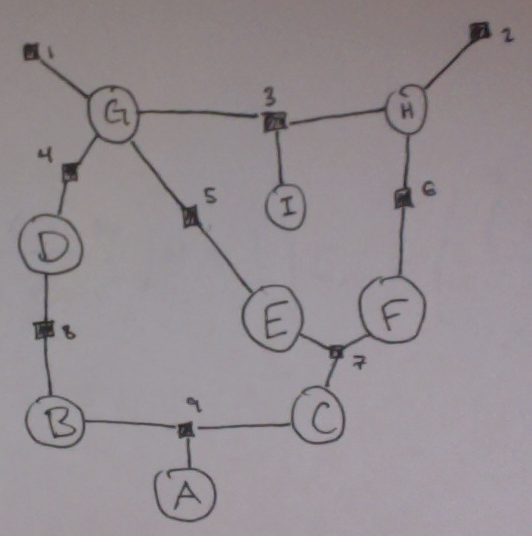
\includegraphics[width=100mm]{factor_graph_a.png}
\end{center}

\begin{center}
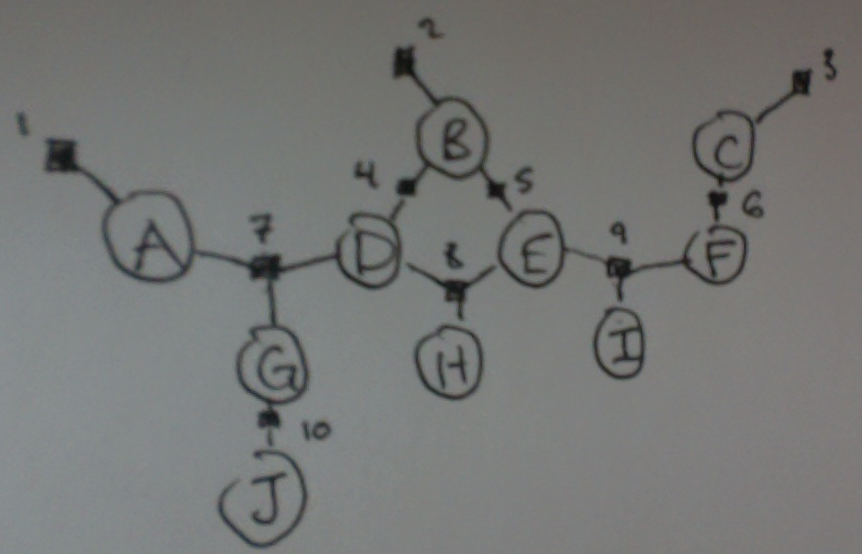
\includegraphics[width=100mm]{factor_graph_b.png}
\end{center}

\subproblem %d

\begin{center}
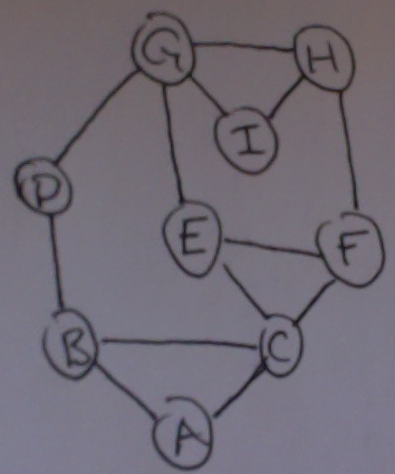
\includegraphics[width=100mm]{undirected_graph_a.png}
\end{center}

\begin{center}
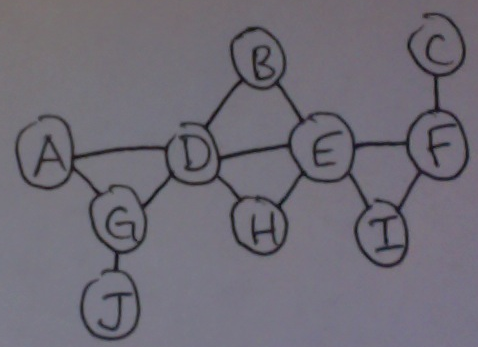
\includegraphics[width=100mm]{undirected_graph_b.png}
\end{center}

%%%%%%%%%%%%%%%%%%%%%%%%%%%%%%%%%%%%%%%%%%%%%%%%%%%%
\problem{25} %3
% Normal(mu, sigma^2)
% (0.2*NormalDistribution[1, 25]) + (0.3*NormalDistribution[-2, 1])+(0.5*NormalDistribution[3, 4])
\subproblem %a
Below is the requested plot of the given density function.
\begin{center}
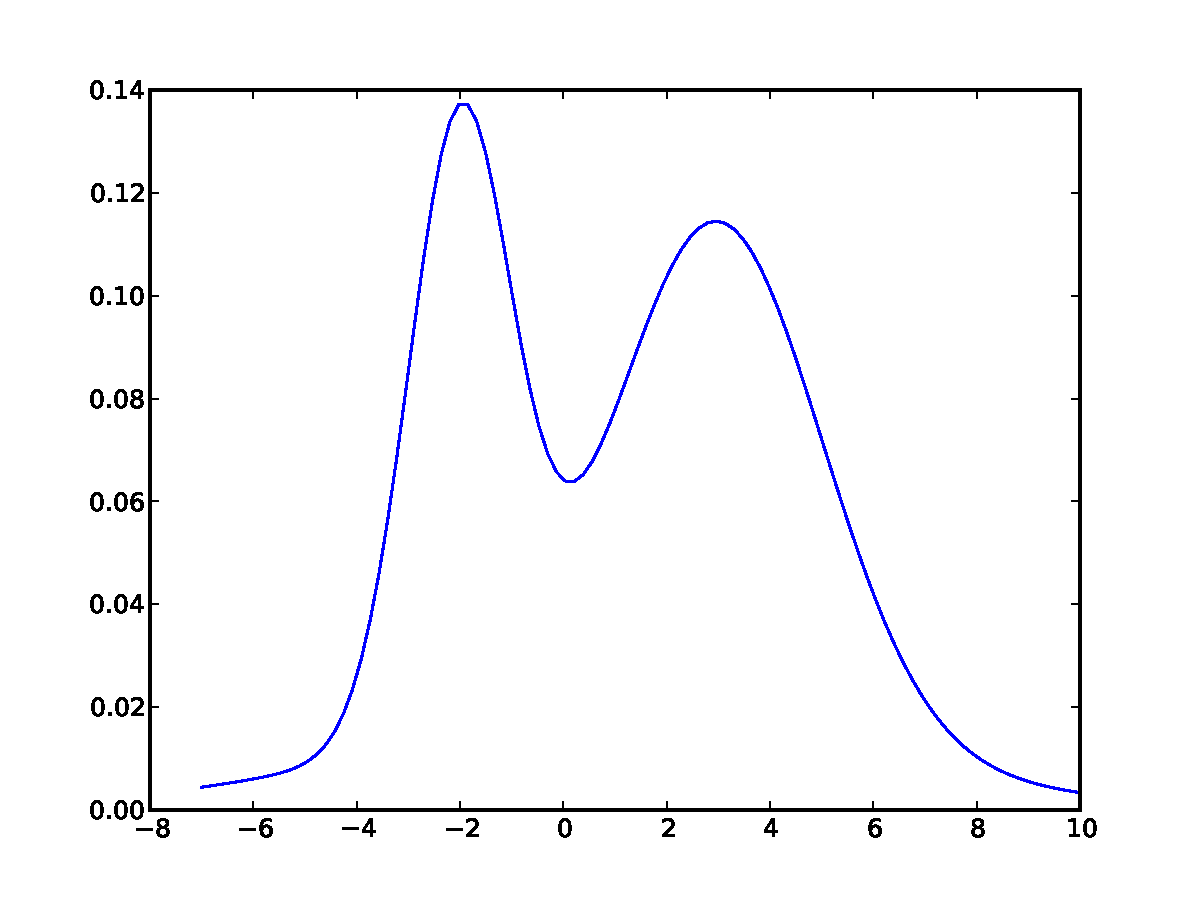
\includegraphics[scale=0.8]{mixture-o-gaussians.pdf}
\end{center}

\subproblem %b
In this problem, we are given three Gaussian densities: $\mathcal{N}(1,25)$, $\mathcal{N}(-2,1)$, and $\mathcal{N}(3,4)$. We are interested in sampling directly from the given mixture of these three Gaussian densities. To generate data directly from the distribution, we use {\tt random.gauss(mu, sigma)}, Python's builtin function for sampling from a Gaussian distribution, and a biased ``three-sided coin." That is, we randomly generate a number between 1 and 10, inclusive. If the number is 1 or 2, we sample from the first Gaussian. If the number is 3, 4, or 5, we sample from the second Gaussian. If the number is 6, 7, 8, 9, or 10, we sample from the third Gaussian distribution. The effect is sampling from the first Gaussian with probability 0.2, from the second Gaussian with probability 0.3, and from the third Gaussian with probability 0.5. Below is a histogram of 500 samples drawn in this way:
\begin{center}
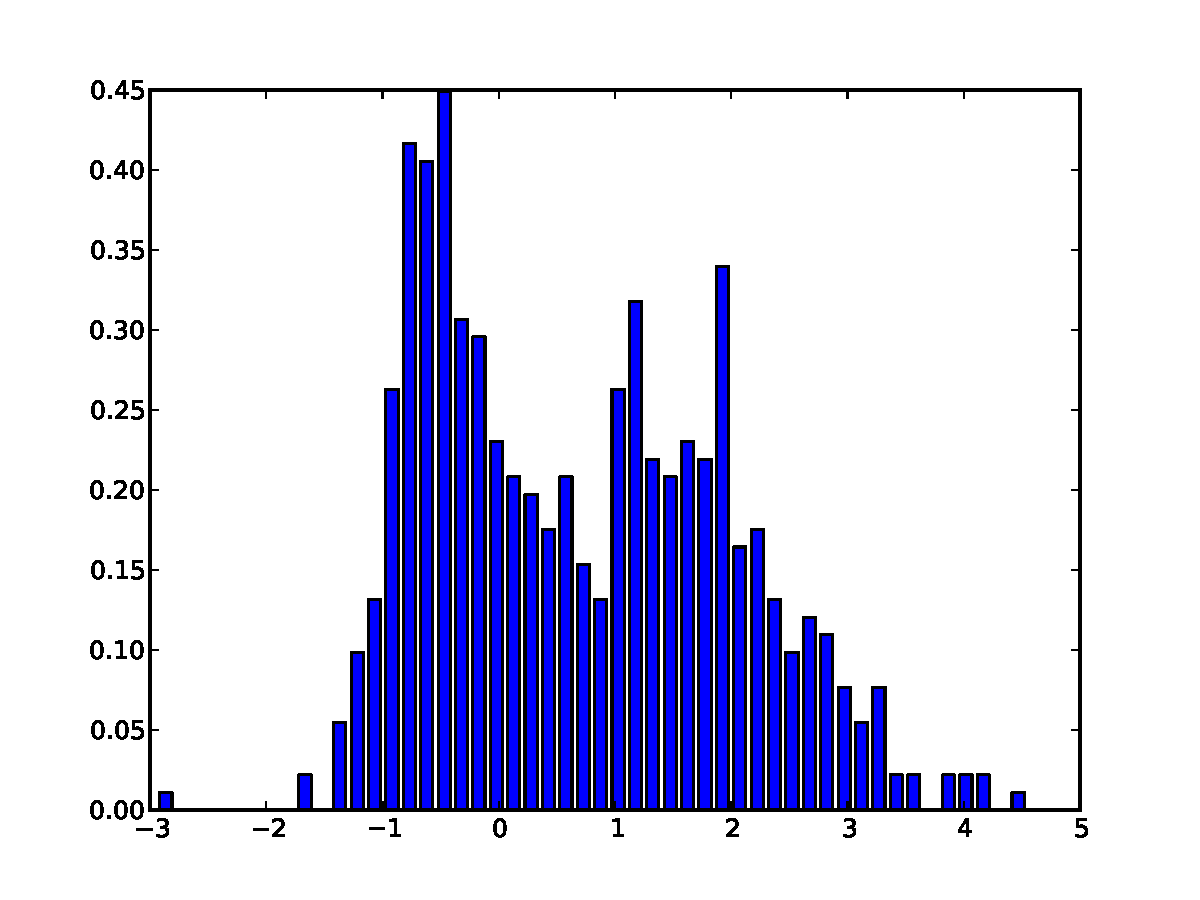
\includegraphics[scale=0.8]{direct-sample-histogram.pdf}
\end{center}

\subproblem %c
In this problem, we pretend we do not know how to perform the ``direct" sampling in (B), and implement a rejection sampler for the given density. We use the upper bounding function $\mathcal{N}(0,24)$ with $c=2$. Below is the requested plot of our upper bounding function against the given density function.
\begin{center}
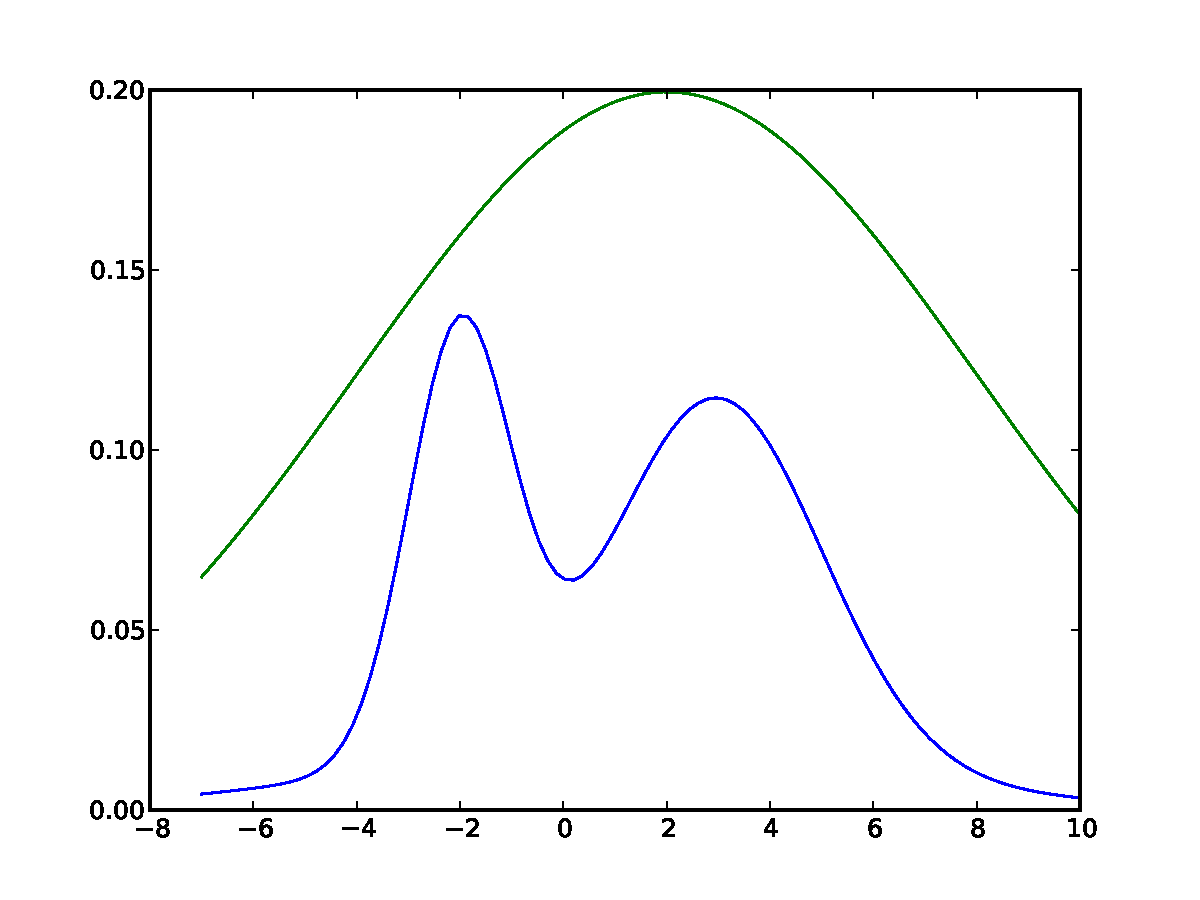
\includegraphics[scale=0.8]{mixture-w-envelope.pdf}
\end{center}

Below is a histogram of 500 samples drawn using our rejection sampler:
\begin{center}
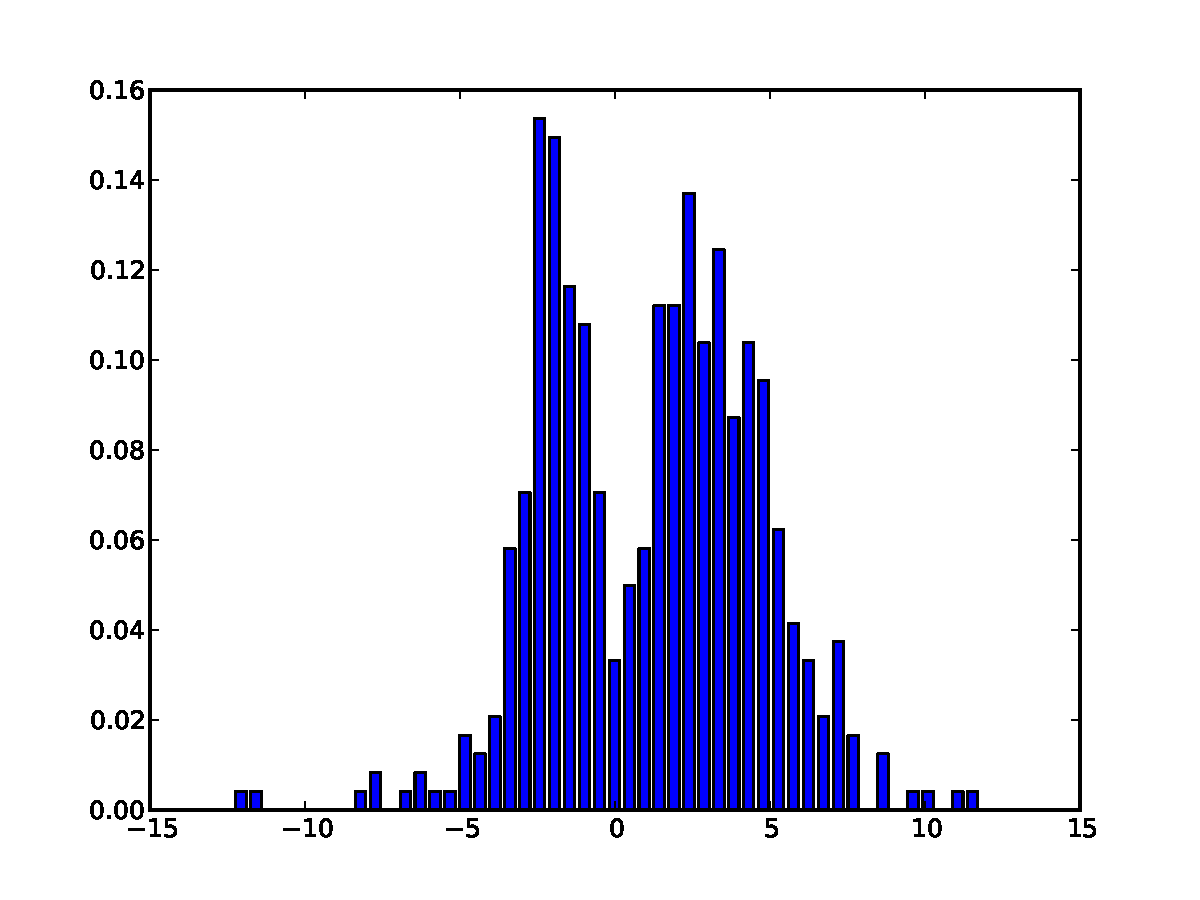
\includegraphics[scale=0.8]{rejection-sample-histogram.pdf}
\end{center}

We got XXX rejections before we got 500 acceptances. This is a X.XX rejection rate.

\subproblem %d\\

We implemented Metropolis-Hastings using a simple Gaussian proposal and a burn in period of 500 samples. 
For our first runs we used a proposal function with a variance of 5 and then we would get an acceptance rate of around 285/500. We then tried a variance of 15 and found that the graph got decidedly worse, also the acceptance rate dropped to 115/500, this graph had more spices.  

\begin{center}
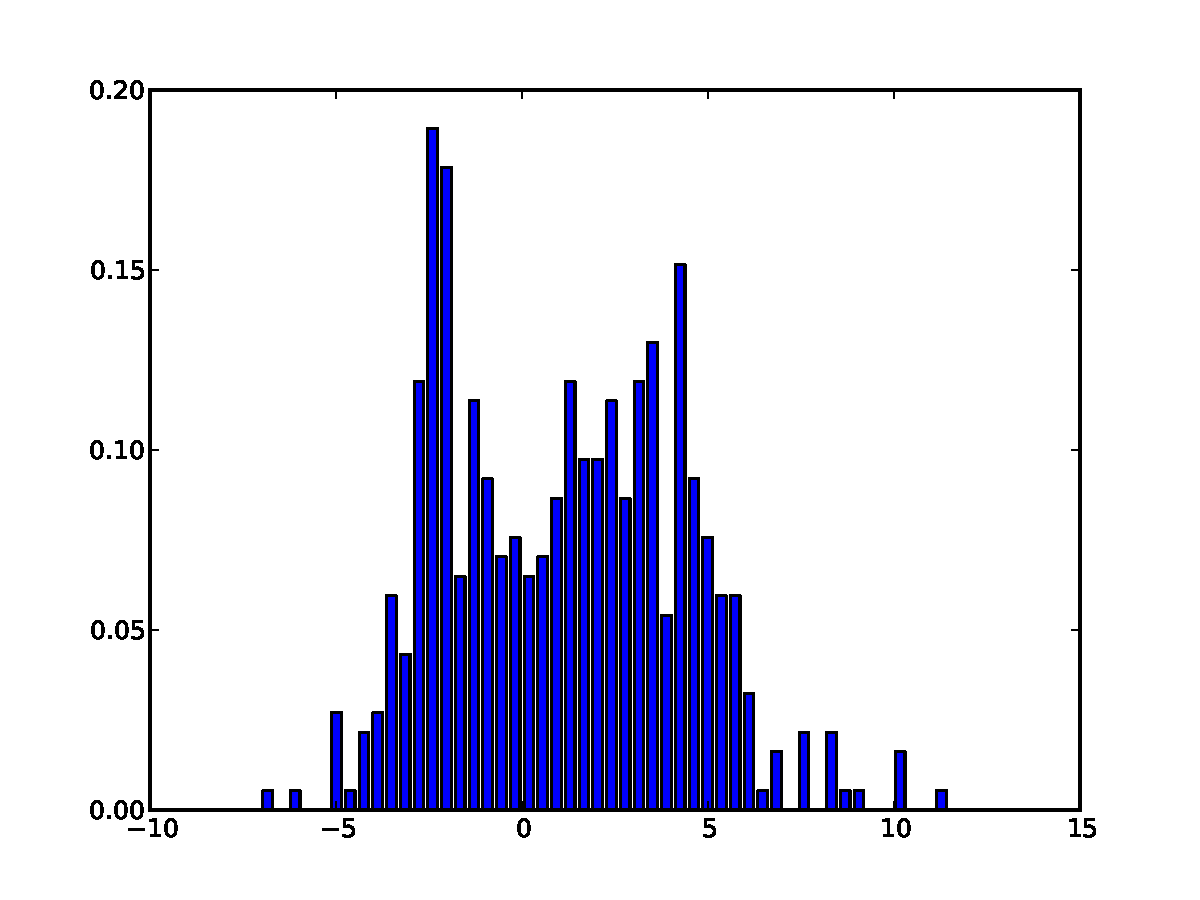
\includegraphics[scale=0.8]{hasty_metro_histogram.pdf}
\end{center}


\end{empfile}

% this invokes metapost on the figures. You must run latex a second
% time for the figures to be included.
\immediate\write18{mpost -tex=latex \jobname}

\end{document}






